\documentclass[conference]{IEEEtran}
\IEEEoverridecommandlockouts
% The preceding line is only needed to identify funding in the first footnote. If that is unneeded, please comment it out.
\usepackage{cite}
\usepackage{amsmath,amssymb,amsfonts}
\usepackage{algorithmic}
\usepackage{graphicx}
\usepackage[spanish]{babel}
\usepackage[utf8]{inputenc}
\usepackage{textcomp}
\usepackage{bm}
\usepackage{mathtools}
\usepackage{xcolor}
\usepackage{multicol}
\usepackage{hyperref}
\usepackage{enumitem}
\usepackage{booktabs}

\def\BibTeX{{\rm B\kern-.05em{\sc i\kern-.025em b}\kern-.08em
    T\kern-.1667em\lower.7ex\hbox{E}\kern-.125emX}}
\newcommand{\norm}[1]{\left\lVert#1\right\rVert}    
\begin{document}

\title{Defensa adversaria en redes neuronales}

\author{\IEEEauthorblockN{Raimundo Becerra}
\IEEEauthorblockA{\textit{Depto. de Ingeniería Eléctrica} \\
\textit{Facultad de Ciencias Físicas y Matemáticas} \\
\textit{Universidad de Chile}\\
Santiago, Chile \\
raimundo.becerra@ing.uchile.cl}
\and
\IEEEauthorblockN{Tomás Saldivia}
\IEEEauthorblockA{\textit{Depto. de Ingeniería Eléctrica} \\
\textit{Facultad de Ciencias Físicas y Matemática}\\
\textit{Universidad de Chile}\\
Santiago, Chile \\
tomas.saldivia@ing.uchile.cl}
}
\maketitle

\begin{abstract} 
El uso de modelos de redes neuronales profundas (DNN) en el mundo real está en un rápido aumento. Acordemente, la preocupación por que estos modelos sean seguros y robustos frente a ataques de adversarios también está en auge, siendo un campo de investigación muy activo. Esto no es de extrañar ya que se ha demostrado que engañar a una DNN es relativamente sencillo: basta resolver un problema de optimización para generar una perturbación en la entrada, siendo esta suficiente para inducir una clasificación incorrecta en el modelo. En este proyecto se propone implementar distintos tipos de ataque, para luego compararlos entre sí en un modelo entrenado con ImageNet. Se proponen además una técnica de defensa a aplicar sobre el modelo, la cual será evaluada para los ataques implementados.
\end{abstract} 

\section{Introducción}
El \textit{deep learning} ha hecho un rápido y significativo progreso en un amplio espectro de áreas dentro del aprendizaje de máquinas, tales como la clasificación de imágenes, el reconocimiento y la detección de objetos, el reconocimiento de voz, síntesis de voz, entre otros \cite{deepdefense}. Esto inevitablemente ha devenido en su aplicación en el mundo físico, especialmente en ambientes y sistemas donde la seguridad es crítica, tales como los vehículos sin conductor, la biometría en cajeros automáticos, etcétera \cite{deepdefense}. Esto, como es de esperar, condujo a la comunidad científica a incurrir en qué tan confiables son estos modelos.

Szegedy \textit{et al.} \cite{goodfellow2013} fue el primero en demostrar que puede ``engañarse'' a un modelo de \textit{deep learning} mediante una pequeña perturbación en la entrada, imperceptible para los seres humanos, generada específicamente con este objetivo. Estas muestras mal clasificadas se denominan \textbf{ejemplos adversarios}. Se ha encontrado que se pueden generar ejemplos adversarios físicos, por ejemplo, para confundir a un automóvil sin conductor mediante la manipulación de una señal de pare, engañando a su sistema de reconocimiento de señales de tránsito \cite{kurakin2016physical, evtimov2017} o mediante la eliminación de la segmentación de peatones en el sistema de reconocimiento de objetos \cite{xie2017}. El generar ejemplos adversarios con el objetivo de engañar a un modelo se conoce como \textbf{ataque adversario}. Un ataque adversario puede ser de tipo caja blanca si es que el adversario conoce los pesos y gradientes del modelo, o de tipo caja negra si es que solo conoce su entrada y salida. Claramente, se hace necesaria la implementación de contramedidas que hagan frente a ataques adversarios, campo de investigación activa que se conoce como \textbf{defensa adversaria}.
% TODO: definir ataques de un paso y múltiples pasos
En este trabajo se busca estudiar distintos métodos de ataque adversario, para luego evaluarlos contra algún método de defensa adversaria. En particular, se proponen los siguientes objetivos: 
\begin{itemize}
	\item Comparar diversos ataques adversarios contra algún modelo de clasificación entrenado con ImageNet, implementando al menos uno.
	\item Implementar una estrategia de defensa adversaria en dicho modelo y analizar su efectividad contra los distintos ataques.
\end{itemize}

Por último, el código utilizado en este proyecto será alojado en GitHub \footnote{Disponible en \url{https://github.com/Tom0497/Adversarial_Defense_In_NN}}. 

\section{Propuesta}

\subsection{Datos}

Los datos a utilizar se extraen de \textit{ImageNet}, una base de datos de imágenes organizada bajo la estructura jerárquica otorgada por \textit{WordNet}, a su vez una base de datos léxica del idioma inglés. Esta última se caracteriza por agrupar palabras en conjuntos de sinónimos los que denomina \textit{synonym set} o \textit{synset}. Luego, \textit{ImageNet} se vale de estos conjuntos para agrupar sus datos, destacando que su objetivo es proveer en promedio 1000 imágenes por \textit{synset}.

A la fecha \textit{ImageNet} cuenta con más de 14 millones de imágenes separadas en más de 20 mil categorías, y desde el año 2010 el equipo detrás de la base de datos realiza una competencia de software donde los participantes presentan sus modelos de clasificación buscando obtener la mayor cantidad de aciertos en esta. El nombre del concurso es \textit{ImageNet Large Scale Visual Recognition Chanllenge (ILSVRC)}, y se caracteriza por limitar la cantidad de categorías que tiene \textit{ImageNet} a 1000. Es importante mencionar que desde fines del año 2017 en adelante, la competencia paso a estar a cargo de la plataformal digital Kaggle, en formato online.

Dado lo anterior, se tiene que los modelos que se entrenan en base a \textit{ImageNet} clasifican imágenes entre 1000 clases. El \textit{dataset} considerado para la competencia se compone de más de un millón de imágenes en el conjunto de entrenamiento, además de tener 50 mil y 100 mil imágenes en los conjuntos de validación y test respectivamente, tomando en conjunto un espacio en memoria de más de 100 GB. Es por esto que se considerarán opciones alternativas para poder solventar la gran cantidad de memoria requerida para albergar los datos.

En general, los datos de entrada a los modelos que utilizan \textit{ImageNet} tienen un tamaño de $224 \times 224$, además de los tres canales de color RGB; pero \textit{ImageNet} provee versiones del \textit{dataset} original con imágenes reducidas en tamaño, implicando un menor uso de memoria para el almacenamiento. Las versiones disponibles son de imágenes de $8\times8$, $16\times16$, $32\times32$ y $64\times64$, en formato RGB. Además de esto, se cuenta con las URLs de las imágenes del \textit{dataset} original correspondiente al ILSVRC 2012, lo que permite descargar algunas de estas sin la necesidad de almacenar el total de los datos.

La cantidad de imágenes y la separación en los distintos conjuntos del \textit{dataset} original se extraen de \cite{imagenet} y se detallan a continuación:

\begin{itemize}
    \item \textbf{Conjunto de entrenamiento:}  1.281.167 imágenes
    \item \textbf{Conjunto de validación} 50.000 imágenes
    \item \textbf{Conjunto de test:} 100.000 imágenes
\end{itemize}

Cabe mencionar que la lista de URLs para descargar las imágenes es proveída por la página oficial de ImageNet, y, como esta corresponde a la competencia del año 2012, se debe tener en cuenta que varios de estos enlaces están caídos debido a diversas causas. Luego, no se asegura la accesibilidad al total de la cantidad de imágenes antes mencionadas.

Cada uno de los objetivos del proyecto se persiguió con un enfoque distinto, debido a que lo que se quiere observar en cada una de esas etapas apunta a distintos fines. Luego, tanto los modelos como los datos específicos utilizados para cada parte difieren, por tanto, se hace imperativo realizar una descripción por separado de los datos utilizados en cada sección. Esto se hace a continuación, teniendo en cuenta que siempre corresponden a subconjuntos de \textit{ImageNet}, variando en sólo en la cantidad de clases y en la cantidad de imágenes por clase.

\subsubsection{Datos para ataques adversarios}

Para probar los ataques adversarios y sus efectos en un modelo, no se requiere de todas las clases y tampoco de muchos ejemplos por clase, mas aún cuando se considera un modelo pre-entrenado para generar ejemplos adversarios, el cual es el caso. Luego, considerando que en la mayoría de los casos la generación adversaria implica el computo de gradientes, se tiene que se reducen la cantidad de clases a considerar, desde las 1000 originales a 50, siendo estas las primeras 50 clases de \textit{ImageNet}. No se especifican las clases debido a que no es relevante saber el nombre de la clase sino más bien los efectos de la generación adversaria sobre la capacidad de clasificación del modelo.

Además de reducir la cantidad de clases, se reduce también la cantidad de imágenes por cada una de estas clases, fijando en 50 ejemplos por cada clase considerada. Luego, se puede observar que el total de imágenes a considerar para esta parte es de 2500 imágenes. Notar que no se especifica ninguna otra división en los datos, esto debido a que no se entrena ningún modelo, sólo se generan ejemplos adversarios.

\subsubsection{Datos para defensa adversaria}

Considerando que para la defensa adversaria se esta obligado en cierto punto a entrenar un modelo, se tiene que reducir considerablemente la imágenes a utilizar, esto tanto para la generación de ejemplos adversarios, pero principalmente para el entrenamiento del modelo. Luego, para tener un entrenamiento viable para un computador doméstico se tienen dos opciones: reducir la cantidad de imágenes, es decir tanto el número de clases como la cantidad de ejemplos por cada una de éstas, ó, reducir el tamaño de las imágenes, considerando quizás algunas de las opciones mencionadas anteriormente respecto a versiones del dataset en versiones de menor tamaño.

Debido a que el proyecto tiene un alto componente visual, en el sentido en que se desean poder observar las distorsiones que sufren las imágenes, se tiene que reducir el tamaño de las imágenes resulta poco práctico para estos fines. Luego, la única opción es reducir la cantidad de imágenes. Para esto se determinó utilizar 3 clases de las 1000 originales, siendo estas: Toucan (clase 96), Digital Clock (clase 530) y Orange (clase 950).

Considerando que todas las clases se crearon balanceadas, y con 500 imágenes cada una, la caracterización de los datos esta dado por:

\begin{itemize}
    \item \textbf{Conjunto de entrenamiento:}  900 imágenes
    \item \textbf{Conjunto de validación} 300 imágenes
    \item \textbf{Conjunto de test:} 300 imágenes
\end{itemize}

\subsubsection{Procesamiento}

Cualquier imagen que se utilice como input para un modelo debe sufrir algún proceso de normalización, esto para limitar los valores de los píxeles en ciertos rangos, evitar sesgos hacia los positivos, etc. En específico, para modelos que utilizan \textit{ImageNet} como base, se tiene que previo a utilizar las imágenes, éstas se estandarizan, es decir, se les resta la media y luego se divide por la desviación estándar, ambos valores calculados sobre los datos de entrenamiento. Esto se realiza píxel a píxel para todas las imágenes, algo que se debe tener en cuenta al momento de visualizar resultados sobre imágenes, debido a que se debe revertir el procesamiento. 

Se debe considerar además que los modelos sobre \textit{ImageNet} en general consideran un input de tamaño $224 \times 224 \times 3$, donde el 3 representa a los canales RGB. Por lo tanto, al leer o descargar cualquier imagen, se debe asegurar de que su tamaño sea el mencionado, por lo que en algunos casos se requiere de ajuste de dimensiones para llegar al tamaño deseado.

\subsection{Modelo}

Al igual que en la parte anterior, la especificación de los modelos utilizados se realiza por secciones, dado que no fue el mismo modelo el utilizado en la primera parte del proyecto que en la segunda. 

Previo a precisar los modelos utilizados es relevante mencionar el software a utilizar y, en específico, las prestaciones útiles para el proyecto. Se tiene que el lenguaje de programación utilizado es Python, y en específico se utiliza la plataforma \textbf{Tensorflow}, para \textit{machine learning}. En términos de las versiones utilizadas, éstas son:
\begin{itemize}
    \item Python 3.7
    \item Tensorflow 1.14
\end{itemize}

\subsubsection{Modelo para ataques adversarios}

El objetivo principal en esta parte es generar ejemplos adversarios, y poder medir como cambia la capacidad de clasificación de un modelo frente a un ataque adversario. Luego, se tiene que el entrenamiento del modelo no es relevante para lo buscado, por lo que se opta por una solución más práctica, la cual corresponde a utilizar un modelo cuyos parámetros ya han sido entrenados sobre el dataset de \textit{ImageNet}. Con esto se asegura que el modelo tiene cierta capacidad de clasificación sobre las imágenes con las que se trabajará, es decir, existe un accuracy base.

La principal ganancia al realizar lo anterior es el ahorro de poder computacional y la posibilidad de utilizar un clasificador de alto nivel. En específico, se utiliza la API de Tensorflow, Keras. Esta se vuelve particularmente útil debido a que cuenta con modelos predefinidos y que en su momento fueron estado del arte en clasificación de imágenes.

Dado esto, se eligió el modelo \textit{ResNet50}. Este modelo fue introducido en el año 2015 y contaba con la característica distintiva de utilizar conexiones residuales entre capas; estos y otros detalles del modelo \textit{ResNet} se pueden consultar en \cite{resnet}. El grafo del modelo se encuentra en el repositorio del GitHub del proyecto, tanto en su versión obtenida de Tensorboard \footnote{Disponible en \url{https://github.com/Tom0497/Adversarial_Defense_In_NN/blob/master/tensorboard_graph.png}}, como conceptual \footnote{Disponible en \url{https://github.com/Tom0497/Adversarial_Defense_In_NN/blob/master/model.png}}.

\subsubsection{Modelo para defensa adversaria}

Se tiene que la defensa de un modelo frente a ataques adversarios requiere de un post entrenamiento o \textit{fine tunning} de los parámetros. Luego, la idea de buscar ahorrar recursos computacionales al utilizar un modelo pre entrenado no se puede aplicar directamente en este apartado, esto debido a que cuando se requiera entrenar al modelo, la cantidad de pesos considerados en una arquitectura como la de \textit{Resnet50} es cercana a los 100 millones, lo que sobrepasa las capacidades de un computador común.

Para solventar lo anterior, se utiliza un funcionalidad de Keras que permite utilizar la parte conformada por bloques convolucionales de una red, es decir, sólo el \textit{feature extractor}, y permitir al usuario acoplar el clasificador al final de los bloques. La ventaja de lo anterior es que se pueden utilizar los pesos pre entrenados, esto implica que para obtener un clasificador con esta arquitectura sólo basta entrenar la red que se acople al final, dado que los pesos ya entrenados se congelan y por tanto, todos esos gradientes no son necesarios de calcular, lo que hace el entrenamiento del modelo mucho más rápido.

Dado lo anterior, se elige como modelo clasificador a VGG16, el cual fue presentado en 2015 por Simonyan
y Zisserman, y al momento de su publicación era el estado del arte en la competencia \textit{ILSVRC} \cite{vgg16}. Se eligió este modelo por sobre Resnet50 debido a que al haber disminuido la cantidad de clases de 1000 a 3 se cree no es necesario una arquitectura tan compleja como la de Resnet para lograr buenos resultados en clasificación.

La arquitectura del modelo utilizado esta dada por:

\begin{table}[!t]
    \centering
    \caption{Arquitectura de la red convolucional implementada para la tarea de defensa adversaria.}
    \label{defense_model}
    \begin{tabular}{c} 
    \toprule 
    Configuración de Red
    \midrule
     conv3-64 \\ conv3-64 
    \bottomrule
    \end{tabular}
\end{table}

\subsection{Generación adversaria}
Se compararán cuatro algoritmos para la generación de ejemplos adversarios: \textit{Fast Gradient Sign Method} \cite{goodfellow2014}, \textit{Fast Gradient Method} \cite{kurakin2016}, \textit{Random Fast Sign Gradient Method} \cite{tramer2017}, \textit{One-Step Least Likely Class} \cite{kurakin2016} y \textit{DeepFool} \cite{deepfool}. Los cuatro primeros se denominan ataques de un paso, es decir, realizan solo un cálculo de gradiente, mientras que el último es un ataque iterativo, pues se calculan iterativamente varios gradientes \cite{kurakin2016} para obtener el ejemplo adversario. Antes de mostrar la teoría subyacente a estos algoritmos, se debe establecer notación. Dado un modelo de \textit{deep learning} ya entrenado $f$, con pesos $\bm{\theta}$, se notará por $\bm{x}$ a alguna entrada, y por $y$ a la etiqueta de esta, con $f(\bm{x})=y$. Dado un ejemplo adversario $\bm{x}'$ tal que $f(\bm{x}')=y'$ con $y \neq y'$, se define $\bm{\eta} = \bm{x}' - \bm{x}$ como la perturbación añadida a $\bm{x}$. Con esto se tiene que, en general, el generar un ejemplo adversario $\bm{x}'$ puede ser descrito como el problema de optimización con restricciones \cite{yuan2017}:
\begin{equation}\label{problemaoriginal}
	\begin{aligned}
		\min_{\bm{x}'} \quad&\norm{\bm{x'}-\bm{x}} \\
	\text{s.t.} \quad &f(\bm{x'})=y'\\
	&f(\bm{x})=y \\
	&y \neq y'
\end{aligned}
\end{equation}
Este problema de optimización minimiza la perturbación manteniendo la clasificación errónea de la predicción para la entrada. Todos los algoritmos de ataque adversario buscan encontrar o al menos aproximarse a la solución de (\ref{problemaoriginal}). 
\begin{itemize}
	\item \textbf{\textit{Fast Gradient Sign Method (FGSM):}} Este ataque consiste en realizar un paso de actualización del gradiente en la dirección del signo del gradiente en cada píxel. La perturbación puede entonces ser expresada como:
		\begin{equation}\label{fgsm_noise}
			\bm{\eta}=\epsilon\cdot \text{sign}(\nabla_{\bm{x}}J(\bm{\theta}, \bm{x}, y))
		\end{equation}
donde $\epsilon$ corresponde a un hiperparámetro ajustable que define la magnitud de la perturbación.
\item \textbf{\textit{Fast Gradient Method (FGM):}} También conocido como \textit{Fast Gradient} $L_2$ \cite{kurakin2016}, es un ataque es similar a $FGSM$, pero en vez de realizar la perturbación de (\ref{fgsm_noise}), se usa el valor del gradiente normalizado:
	\begin{equation}\label{fgm_noise}
	\bm{\eta}=\epsilon\cdot \frac{\nabla_{\bm{x}}J(\bm{\theta}, \bm{x}, y)}{\norm{\nabla_{\bm{x}}J(\bm{\theta}, \bm{x}, y)}_2}
	\end{equation}
Esto significa que se realiza un paso de actualización del gradiente en la dirección de este en cada píxel.
% FALTA AGREGAR JUSTIFICACION DE FGM
\item \textbf{\textit{Random Fast Gradient Sign Method (R-FGSM):}} Otro método similar a \textit{FGSM}, pero en el que se agrega una componente aleatoria, lo cual tiene como consecuencia que es un método de ataque \textit{black-box} más efectivo que \textit{FGSM} \cite{tramer2017}. Para un ejemplo $\bm{x}$, este ataque genera un ejemplo adversario $\bm{x'}$ según:
	\begin{equation}
		\bm{x'}=\bm{\hat{x}} + (\epsilon - \alpha) \cdot \text{sign}(\nabla_{\bm{\hat{x}}} J(\bm{\theta}, \bm{\hat{x}}, y))
	\end{equation}
	donde $\bm{\hat{x}}$ está dado por
\begin{equation}
\bm{\hat{x}}=\bm{x} + \alpha \cdot \text{sign}(\bm{\xi})
\end{equation}
siendo $\bm{\xi}\sim\mathcal{N}(\bm{0}, \text{\textbf{I}})$ una variable aleatoria que distribuye según una gaussiana multidimensional acorde a las dimensiones de la imagen y $\alpha, \epsilon$ hiperparámetros, con $\alpha < \epsilon$.

\item \textbf{\textit{One-Step Least Likely Class (step l.l.):}} A diferencia de los métodos anteriores, este método es un \textit{targeted attack}, es decir, el ejemplo adversario maximiza la probabilidad de que el modelo prediga una clase en específica. En este caso, se maximizará la probabilidad de que el modelo prediga la clase de menor probabilidad. La perturbación para obtener el ejemplo adversario será:
\begin{equation}\label{stepll_noise}
	\bm{\eta}=-\epsilon\cdot \text{sign}(\nabla_{\bm{x}}J(\bm{\theta}, \bm{x}, y_{LL}))
\end{equation}
donde $y_{LL}=\arg \min_{y} p(y | \bm{x}; \bm{\theta})$ es la clase de menor probabilidad. Notar que a diferencia de (\ref{fgsm_noise}) y (\ref{fgm_noise}), el signo de la perturbación en (\ref{stepll_noise}) es negativo.
\item \textbf{\textit{DeepFool (DF):}} A diferencia de los ataques anteriores, este ataque es iterativo. Para generar un ejemplo adversario, busca la mínima distancia desde el input a la frontera de decisión más cercana y para sobrellevar la no-linealidad en altas dimensiones realiza una optimización iterativa en conjunto con una aproximación lineal. Si se considera un clasificador binario $f$, el cual hace sus predicciones según el signo de su output, se tiene que la perturbación de este ataque está dada por $\bm{\eta}=\bm{r}^{(0)} + ... + \bm{r}^{(n-1)}$, donde el $i$-ésimo sumando $\bm{r}^{(i)}$, para $i=0,...,n-1$, se obtiene aplicando el teorema de Taylor y resolviendo:
	\begin{align}
		\min_{\bm{r}} \norm{\bm{r}}_{2} \quad \text{ s.t. } f(\bm{x} + \bm{\eta}^{(i)}) + \nabla_{\bm{x}}f(\bm{x}+\bm{\eta}^{(i)})^{T}\bm{r}=0
		\label{deepfoolmin}
	\end{align}
	en donde $\bm{\eta}^{(i)} \coloneqq \sum_{j=0}^{i-1}\bm{r}^{(j)}$. Es fácil ver que (\ref{deepfoolmin}) tiene la solución analítica: 
\begin{equation}
	\bm{r}^{(i)} = -\frac{f(\bm{x} + \bm{\eta}^{(i)})}{\norm{\nabla_{\bm{x}} f(\bm{x} + \bm{\eta}^{(i)})}^{2}_{2}} \nabla_{\bm{x}} f(\bm{x} + \bm{\eta}^{(i)})
	\end{equation}
Si en alguna iteración se obtiene que $\text{sign}(f(\bm{x}+\bm{\eta}^{(i)})) \neq \text{sign}(f(\bm{x}))$, entonces se detiene el algoritmo y se retorna la perturbación encontrada. Esta estrategia puede extenderse a clasificadores de múltiples clases, lo que requiere encontrar la frontera de decisión más cercana y utilizar la clase adyacente a esta frontera como clase objetivo de la minimización \cite{deepdefense, yuan2017}.
\end{itemize}

Una vez definidos los ataques propuestos, se procederá a justificar su elección. \textit{FGSM} se elige ya que es el tipo de ataque más popular, es simple y fue el primero en poder ser utilizado de manera práctica; esto lo ha transformado en una especie de ataque ``benchmark'', con el cual los nuevos ataques son comparados para corroborar su validez. \textit{FGM} se escoge ya que es un método simple de implementar una vez ya implementado \textit{FGSM} y sería interesante comparar ambos ataques. De la misma forma, \textit{R-FGSM} también es fácil de implementar una vez ya implementado \textit{FGSM}, además de que se encontró en \cite{tramer2017} que \textit{R-FGSM} es robusto tanto como ataque \textit{black-box} como ataque \textit{white-box}, mientras que \textit{FGSM} solo es robusto como este último, por lo que \textit{R-FGSM} será especialmente útil para realizar los experimentos con los modelos de caja negra. En cuanto al único ataque \textit{targeted}, \textit{step l.l.}, se escogió este ya que \cite{kurakin2016} encontró que era el ataque que mayor robustez concedía a los modelos Inception v3 al utilizar sus ejemplos adversarios como entradas del entrenamiento (\textit{adversarial training}). \textit{DF} se elige debido a ser uno de los métodos iterativos más simples, además de que se ha encontrado que hacer \textit{fine-tuning} en modelos entrenados con ImageNet con ejemplos adversarios generados con \textit{DF} mejora la robustez de los modelos frente a ataques \textit{DF} y \textit{FGSM} \cite{deepdefense}.

Se implementarán \textit{FGSM}, \textit{FGM}, \textit{R-FGSM} y \textit{step l.l.} en Python, utilizando la API de Tensorflow, Keras. Para \textit{DF}, en cambio, se utilizará la librería de Python especializada en ataque adversario, \textit{Foolbox} \cite{foolbox}. 
\subsection{Defensa adversaria}
Para mejorar el rendimiento de modelos frente a ataques adversarios, se propone implementar la técnica de inyectar ejemplos adversarios en el conjunto de entrenamiento del modelo, denominada \textit{adversarial training}. Esta técnica fue descrita por primera vez en \cite{goodfellow2014} pero solo probó su efectividad en datasets pequeños (MNIST y CIFAR10). En \cite{kurakin2016} se mostró que esta técnica también es efectiva en modelos entrenados con ImageNet, pero solo contra ataques de un paso (tales como \textit{FGSM} y \textit{R-FGSM}). En cuanto a \textit{DeepFool}, en \cite{deepdefense} se definió un nuevo tipo de \textit{adversarial training}, bautizado como \textit{Deep Defense}, y se encontró que al usar esta técnica con ejemplos adversarios generados con \textit{DF} aumenta la robustez de modelos entrenados con ImageNet frente a este mismo tipo de ataque. Se procederá a definir entonces las técnicas de \textit{adversarial training}, según lo expuesto en \cite{kurakin2016}, y \textit{Deep Defense}, según \cite{deepdefense}.
\begin{itemize}
	\item \textbf{\textit{Adversarial training:}} En primer lugar, se recomienda utilizar \textit{batch normalization} para realizar esta técnica en ImageNet. Para esto es importante que tanto ejemplos normales como adversarios sean agrupados en el batch antes de realizar un paso de entrenamiento. Para un batch de tamaño $m$ y un número $k$ de ejemplos adversarios en este, la agrupación se realiza de la siguiente forma:
		\begin{enumerate}
			\item Se lee el batch $B=\{\bm{x}_1,\dots,\bm{x}_m\}$ del training set.
			\item Se generan $k$ ejemplos adversarios $\{\bm{x'}_1,\dots,\bm{x'}_k\}$ a partir de los ejemplos normales $\{\bm{x}_1,...,\bm{x}_k\}$ usando el estado actual del modelo $f$.
			\item Se genera un nuevo batch $B'=\{\bm{x'}_1,\dots,\bm{x'}_k,\bm{x}_{k+1},\dots,\bm{x}_m\}$.
			\item Se realiza un paso de entrenamiento en el modelo $f$ usando el batch $B'$.
		\end{enumerate}
Los pasos anteriores se repiten hasta que el entrenamiento converja, siendo el estado inicial del modelo $f$ aleatorio (o con los pesos del modelo ya entrenado, en caso de querer hacer \textit{fine-tuning}). Además, se usa la siguiente función de pérdida que permita el control independiente del número relativo de ejemplos adversarios en cada batch:
\begin{equation}
	\frac{1}{(m-k) + \lambda k}\bigg( \sum_{i \in I} L(y_i, f(\bm{x}_i)) + \lambda \sum_{i \in I'} L(y_i, f(\bm{x'}_i)) \bigg)
\end{equation}
donde $I=\{{k+1},\dots,m\}$ y $I'=\{1,\dots,k\}$ corresponden a los índices de los ejemplos normales y adversarios del batch $B'$, respectivamente; $L(y, f(\bm{x}))$ corresponde a la pérdida de un solo ejemplo $\bm{x}$ con etiqueta $y$ y $\lambda$ es el parámetro que controla el peso relativo de los ejemplos adversarios en la pérdida. Se observó en \cite{kurakin2016} que si se escoge un valor de $\epsilon$ específico para el entrenamiento, el modelo solo se vuelve robusto contra ataques generados con este valor de $\epsilon$, por lo que se recomienda escoger $\epsilon$ aleatoria e independientemente en cada ejemplo de entrenamiento. En \cite{kurakin2016} los mejores resultados se obtuvieron al elegir una distribución normal truncada, definida en el intervalo [0, 16] y con distribución subyacente $\mathcal{N}(0, 8)$.
\item \textbf{\textit{Deep Defense:}} Esta técnica es descrita en \cite{deepdefense}, pero solo a nivel de la función de pérdida a utilizar en el entrenamiento. Como no se especifica qué batch utilizar, se propone la siguiente metodología:
\begin{enumerate}
			\item Se lee el batch $B=\{\bm{x}_1,...,\bm{x}_m\}$ del training set.
			\item Se generan $m$ ejemplos adversarios $\{\bm{x'}_1,...,\bm{x'}_m\}$ a partir de los ejemplos normales $\{\bm{x}_1,...,\bm{x}_m\}$ usando el estado actual del modelo $f$. Es decir, a cada ejemplo normal le corresponde un ejemplo adversario.
			\item Se realiza un paso de entrenamiento en el modelo $f$ usando el batch $B$ y utilizando la función de pérdida característica de \textit{Deep Defense}.
		\end{enumerate}
Los pasos anteriores se repiten hasta que el entrenamiento converja, inicializando los pesos de $f$ de manera aleatoria (o con los pesos del modelo ya entrenado, en caso de querer hacer \textit{fine-tuning}). La función de pérdida característica de este método será:
\begin{equation}\label{eq:deepdefenselossfunction}
	\sum_{i=1}^m L(y_i, f(\bm{x}_i)) + \mu \sum_{i=1}^m R\bigg( -\frac{\norm{\bm{x'}_i - \bm{x}_i}_p}{\norm{\bm{x}_i}_p}  \bigg)
\end{equation}
donde se ha usado una regularización basada en el parámetro $\norm{\bm{x'}-\bm{x}}_p$, i.e. la $p$-norma ($p \in [1, \infty)$) de la perturbación, normalizado por $\norm{\bm{x}}_p$; y la constante de regularización $\mu$. La función $R$ debe tratar a los ejemplos clasificados correcta e incorrectamente de manera diferente y ser monótonamente creciente en estos últimos (por ejemplo, $R(t) = \exp(t)$). Esta función de pérdida no asegura que no disminuya el \textit{accuracy} de los ejemplos, por lo que se recomienda tratar de forma distinta a los ejemplos cuya versión adversaria engaña y no engaña al modelo. Para esto, el segundo sumando de (\ref{eq:deepdefenselossfunction}) se reemplaza por
\begin{equation}
	\mu \sum_{i \in \mathcal{T}} R \bigg( -c\frac{\norm{\bm{x'}_i - \bm{x}_i}_p}{\norm{\bm{x}_i}_p}  \bigg) + \mu \sum_{i \in \mathcal{F}} R \bigg( d\frac{\norm{\bm{x'}_i - \bm{x}_i}_p}{\norm{\bm{x}_i}_p}  \bigg)
\end{equation}
donde $c,d > 0$ son dos factores de escala que balancean la importancia de las muestras, $R$ se escoge como la función exponencial y $\mathcal{T}, \mathcal{F}$ se definen como
\begin{align}
	\mathcal{T}=\{ i\in J | f(\bm{x}_i) = y_i \}\\
\mathcal{F}=\{ i\in J  | f(\bm{x}_i) \neq y_i \} \end{align}
donde $J=\{ 1,\dots, m \}$, es decir, son los índices de los ejemplos normales bien y mal clasificados, respectivamente, por el modelo en su estado actual.
\end{itemize}
Para la implementación de estas dos técnicas se utilizará la API de Tensorflow, Keras. Para \textit{Deep Defense} específicamente, se utilizará como guía la implementación provista por \cite{deepdefense}, la cual utiliza el framework PyTorch \footnote{Disponible en \url{https://github.com/ZiangYan/deepdefense.pytorch/}}. 
%\subsubsection{Justificación}
%Definición y justficiación del tipo de algoritmo a usar.
%\subsubsection{Principio de optimización}
%Definición de salidas deseadas, función objetivo, principio de optimización a usar.
%\subsubsection{Listado de parámetros}
%Criterio de detención del algoritmo, listado de parámetros e hiperparámetros por definir y/o ajustar.
%\subsubsection{Software}
%Definición del software a usar, definiri qué aspectos se programarán y en qué lenguaje (e.g. rutinas complelentarias a un toolbox específico).
\section{Resultados esperados}
\subsection{Ataque adversario}
Para comparar los distintos tipos de ataques adversarios, se utilizará el \textit{accuracy} top-1 y top-5. El primero es el \textit{accuracy} común y corriente, i.e. la proporción de imágenes correctamente clasificadas con máxima probabilidad por el modelo. El segundo es la proporción de imágenes cuya etiqueta correcta está entre las 5 etiquetas predichas con máxima probabilidad por el modelo. Ambas medidas de \textit{accuracy} serán calculadas sobre imágenes adversarias generadas por los distintos ataques y comparadas con el \textit{accuracy} para el total de ejemplos limpios, lo cual será presentado en una tabla. 

Se espera que \textit{DeepFool} tenga 0\% de \textit{accuracy} top-1, pues el algoritmo está diseñado para encontrar la perturbación necesaria para una clasificación incorrecta. El resto de los ataques, todos de un paso y basados en el gradiente, tienen como hiperparámetro $\epsilon$, por lo cual no se puede asegurar 0\% de \textit{accuracy} top-1 a menos que se busque activamente, por cada imagen, el $\epsilon$ necesario para que la perturbación provoque una clasificación errónea. De todos modos, se espera un \textit{accuracy} top-1 mucho menor al del modelo con ejemplos normales. En esta misma línea, un recurso gráfico útil para comparar distintos ataques de un paso es graficar el hiperparámetro $\epsilon$ contra el top-1 y top-5 \textit{accuracy}, como se ve en el apéndice de \cite{kurakin2016}.
\subsection{Defensa adversaria}
Para medir qué tan efectiva es la defensa adversaria, se utilizarán las métricas propuestas en \cite{deepdefense}: para los ataques con \textit{FGSM} y sus derivados se utilizará \textit{accuracy} top-1 en el conjunto de validación perturbado y para ataques \textit{DeepFool} se utilizará la denominada \textit{robustness}, definida por primera vez en \cite{deepfool} como:
\begin{equation}
\rho_p \coloneqq \frac{1}{|\mathcal{V}|} \sum_{i \in \mathcal{V}} \frac{\norm{\bm{\eta}_i}_p}{\norm{\bm{x}_i}_p}
\end{equation}
para algún $p\in [0, \infty)$ que define la norma a utilizar y siendo $\mathcal{V}$ los índices del conjunto de validación. 

Para \textit{adversarial training} y según lo expuesto en \cite{kurakin2016}, se espera que el modelo más robusto, al menos contra ataques de un paso, sea el entrenado con ejemplos adversarios generados con \textit{step l.l.}. En cuanto a ataques iterativos como \textit{DF}, \textit{adversarial training} con ejemplos generados en un paso no es efectivo como defensa. En \cite{kurakin2016} también se intentó hacer \textit{adversarial training} con ejemplos generados iterativamente pero los resultados no fueron beneficiosos, por lo que se espera que entrenar con \textit{DF} no necesariamente mejore la robustez del modelo.

Con \textit{Deep Defense} se espera mejorar el \textit{robustness} frente a ataques \textit{DF} del modelo, teniendo como referencia que en \cite{deepdefense} se alcanzó una mejora en este parámetro de un $1.5\%$ en los modelos AlexNet y ResNet-18, además de que se mejoró ligeramente el \textit{accuracy} en los ejemplos normales del conjunto de validación. Por otro lado, no se tiene una referencia qué tan bien rinde \textit{Deep Defense} contra ataques de un paso en modelos entrenados con ImageNet.

%Resultados esperados, medidas de desempeño a usar para evaluar los modelos, forma en que se presentarán los resultados (tablas y gráficos).
%thefinding that multi-step attack methods are somewhat less transferable than single-step attack methods, so single-step attacks are the best for mounting black-box attacks (Kurakin, 2016)
\section{Recursos computacionales}
En primer lugar se estimará el tiempo que tomaría obtener ejemplos adversarios para los distintos ataques de un único paso (en total 4), siendo $n$ el número de ejemplos adversarios a generar por cada ataque de este tipo, $c$ el número de valores de $\epsilon$ a utilizar y asumiendo que el tiempo de todos los ataques de un paso demoran un tiempo $t_{\text{step}}$ constante en generar un ejemplo adversario, entonces el tiempo total de computación será:
\begin{equation}\label{tiempocomputo}
    t_{T} = 4nct_{\text{step}}
\end{equation}
En experimentos preliminares se utilizó Google Colab para la generación de ejemplos adversarios, iterándose en un for-loop las distintas imágenes. Se encontró experimentalmente que el $t_{\text{step}}$ no es constante a través de las iteraciones, y de hecho crece linealmente respecto a estas. Esto es inesperado y como solución momentánea, solo se entrenaron conjuntos de 50 imágenes en cada for-loop, teniendo que reiniciar el entorno de ejecución de Colab una vez terminado el loop para que el tiempo de ejecución volviera a su estado original (el cual era de alrededor de 5 segundos). En la Figura \ref{tiempoejecucion} se muestra este fenómeno para 50 imágenes, utilizando el ataque \textit{R-FGSM}.
\begin{figure}[!t]
    \centering
    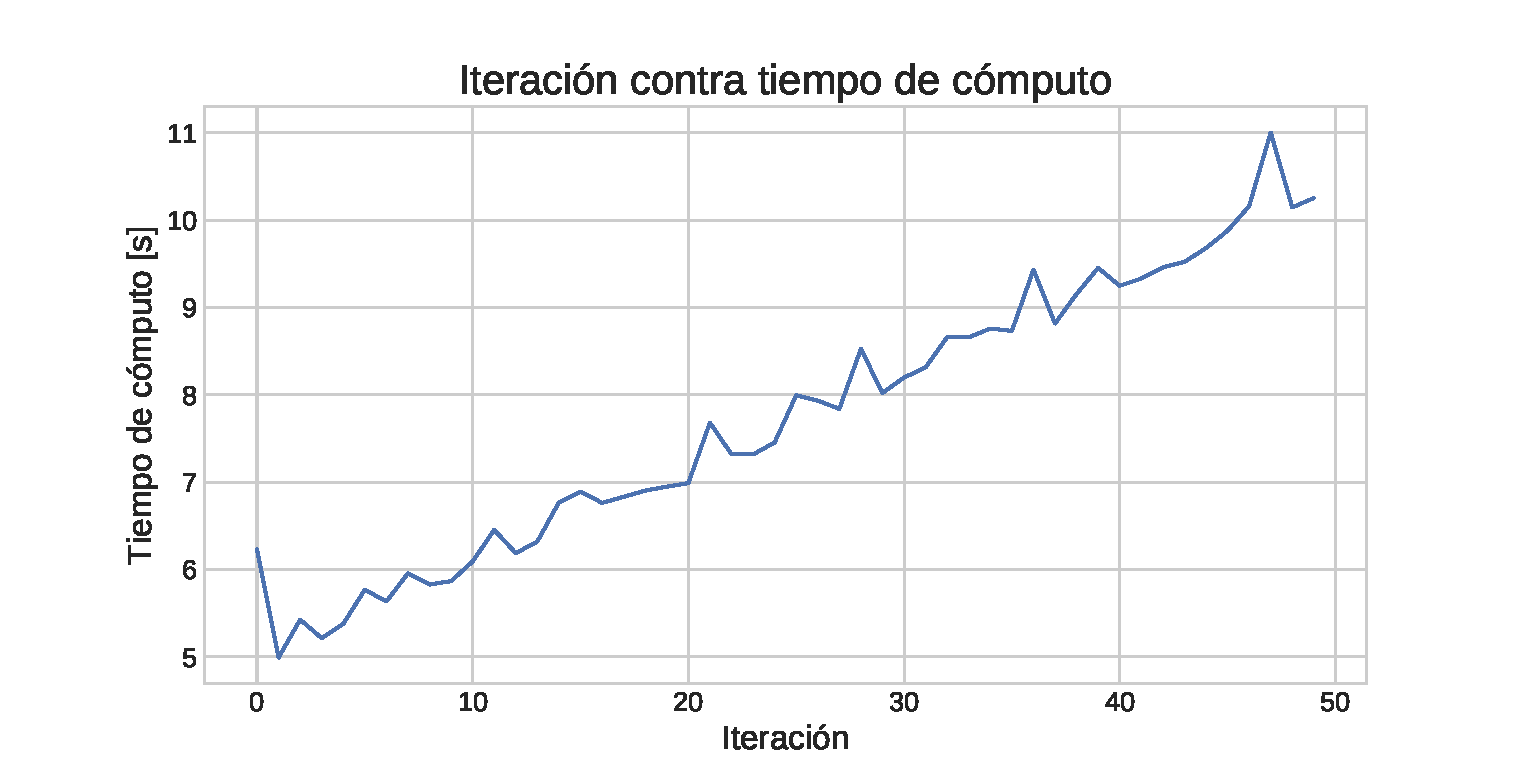
\includegraphics[width=\linewidth]{tiempo_de_computo.eps}
    \caption{Evolución del tiempo de cómputo para 50 imágenes adversarias. Ataque \textit{R-FGSM}.}
    \label{tiempoejecucion}
\end{figure}
Con este fenómeno, (\ref{tiempocomputo}) quedaría mejor enunciada como
\begin{equation}\label{tiempocomputo2}
    t_{T} = 4c \sum_{i=1}^n ( a i + b ) = 4cn\bigg(a\frac{(n+1)}{2} + b\bigg)
\end{equation}
para ciertas constantes $a,b$. Experimentalmente se encuentra que estas son del orden de $a=0.1$ y $b=5$. Claramente, con este comportamiento, se pasa de un problema de complejidad $O(n)$ en (\ref{tiempocomputo}) a uno de $O(n^2)$ en (\ref{tiempocomputo2}). En los experimentos preliminares, se utilizó $n=50$ y $c=5$. Con (\ref{tiempocomputo2}) se obtiene un tiempo total de 7550 segundos, aproximadamente 2 horas. Si se considera un $t_{\text{step}}$ constante igual a 5 segundos, y se utiliza (\ref{tiempocomputo}), se obtiene un tiempo total de 5000 segundos, aproximadamente 1 hora y 20 minutos. Es necesario entonces resolver este problema, pues los métodos de \textit{adversarial training} requieren generar muchos más ejemplos y esto no es viable con un tiempo de cómputo creciente. 
%acionales, número y tiempo de simulaciones a realizar para completar los experimentos necesarios que cumplen los objetivos.

\section{Planificación}
Para la realización del proyecto, se ha divido el trabajo a realizar en metas u objetivos, los cuales se muestran a continuación. Para cada uno de ellos se asigna un tiempo estimativo de trabajo efectivo como también, dado esto y la disponibilidad de tiempo de los integrantes, una fecha tentativa de inicio y fin. 

\begin{enumerate}
    \item \textit{}{Extracción y procesamiento de datos:} 
        \begin{itemize}
        \item \textbf{Horas de trabajo:} 30 horas
        \item \textbf{Inicio:}  9 de septiembre
        \item \textbf{Término:} 27 de septiembre
    \end{itemize}
    \item \textit{Implementación de ataques adversarios:} 
        \begin{itemize}
        \item \textbf{Horas de trabajo:} 20 horas
        \item \textbf{Inicio:} 25 de septiembre
        \item \textbf{Término:} 4 de octubre
    \end{itemize}
    \item \textit{Realizar experimentos de generación de ejemplos adversarios:} 
    \begin{itemize}
        \item \textbf{Horas de trabajo:} 10 horas
        \item \textbf{Inicio:} 2 de octubre
        \item \textbf{Término:} 5 de octubre
    \end{itemize}
    \item \textit{Implementación de \textit{adversarial training}:}
        \begin{itemize}
        \item \textbf{Horas de trabajo:} 20 horas
        \item \textbf{Inicio:} 7 de octubre
        \item \textbf{Término:} 18 de noviembre
    \end{itemize}
    \item \textit{Implementación de \textit{Deep Defense}:}
        \begin{itemize}
        \item \textbf{Horas de trabajo:} 30 horas
        \item \textbf{Inicio:} 18 de octubre
        \item \textbf{Término:} 1 de noviembre
    \end{itemize}
    \item \textit{Realizar experimentos de defensa adversaria:}
        \begin{itemize}
        \item \textbf{Horas de trabajo:} 10 horas
        \item \textbf{Inicio:} 1 de noviembre
        \item \textbf{Término:} 8 de noviembre
    \end{itemize}
    \item \textit{Implementación de ataques \textit{black-box}:}
        \begin{itemize}
        \item \textbf{Horas de trabajo:} 10 horas
        \item \textbf{Inicio:} 9 de noviembre
        \item \textbf{Término:} 15 de noviembre
    \end{itemize}
    \item \textit{Realizar experimentos de ataques \textit{black-box}:}
           \begin{itemize}
        \item \textbf{Horas de trabajo:} 5 horas
        \item \textbf{Inicio:} 9 de noviembre
        \item \textbf{Término:} 15 de noviembre
    \end{itemize}
    \item \textit{Presentación de resultados y redacción de informe final:}
        \begin{itemize}
        \item \textbf{Horas de trabajo:} 30 horas
        \item \textbf{Inicio:} 1 de noviembre
        \item \textbf{Término:} 22 de noviembre
    \end{itemize}
\end{enumerate}

Cabe destacar que algunas de estas metas ya se han completado, como lo son la extracción y procesamiento de los datos, la implementación de los ataques adversarios, experimentación con generación de ejemplos adversarios.

Los pasos a seguir se centran principalmente en la defensa adversaria, la cual requerirá de la realización de \textit{fine-tuning} sobre algún modelo pre-entrenado de manera tal que este se vuelva resistente o robusto a los ataques adversarios considerados.
%Pasos a seguir para cumpir el objetivo del proyecto al 15 de noviembre, con el número de horas de dedicación a cada etapa del proyecto.

\section{Resultados preliminares}

En primer lugar, se debe tener en cuenta que los ataques adversarios buscan engañar a modelos de clasificación, luego lo primero que se debe tener antes de cualquier experimento, es un modelo de clasificación entrenado. Dado que entrenar un clasificador desde cero puede eventualmente tomar mucho tiempo si no se cuenta con el poder de procesamiento adecuado, se decide por utilizar un modelo pre-entrenado. Para esto, se hace uso de los modelo pre-entrenados que ofrece la API de Tensorflow, Keras, la cual cuenta con más de 10 modelos y sus pesos pre-entrenados.

Dado esto, se eligió el modelo \textit{ResNet50}, aunque no se descarta el uso de algún otro disponible en futuras pruebas. Este modelo fue introducido en el año 2015 y contaba con la característica distintiva de utilizar conexiones residuales entre capas; estos y otros detalles del modelo \textit{ResNet} se pueden consultar en \cite{resnet}. El grafo del modelo se encuentra en el repositorio del GitHub del proyecto, tanto en su versión obtenida de Tensorboard \footnote{Disponible en \url{https://github.com/Tom0497/Adversarial_Defense_In_NN/blob/master/tensorboard_graph.png}}, como conceptual \footnote{Disponible en \url{https://github.com/Tom0497/Adversarial_Defense_In_NN/blob/master/model.png}}.

\subsection{Descripción de experimento}
\begin{figure}[!t]
    \centering
    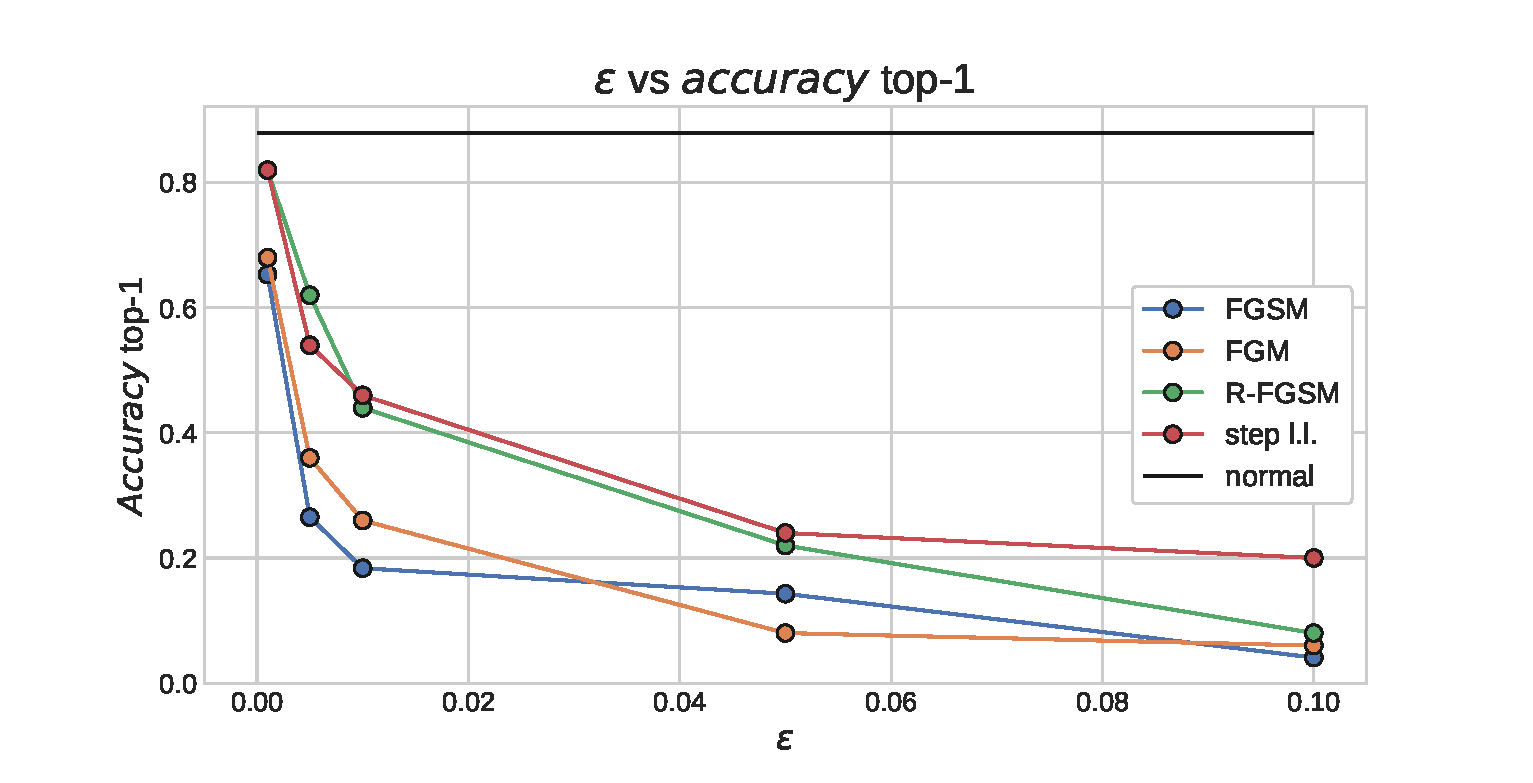
\includegraphics[width=\linewidth]{accuracy_top1.eps}
       \caption{\textit{Accuracy} top-1 contra $\epsilon$, para conjunto de 50 imágenes.}
    \label{fig:accuracytop1}
\end{figure}
\begin{figure}[!t]
    \centering
    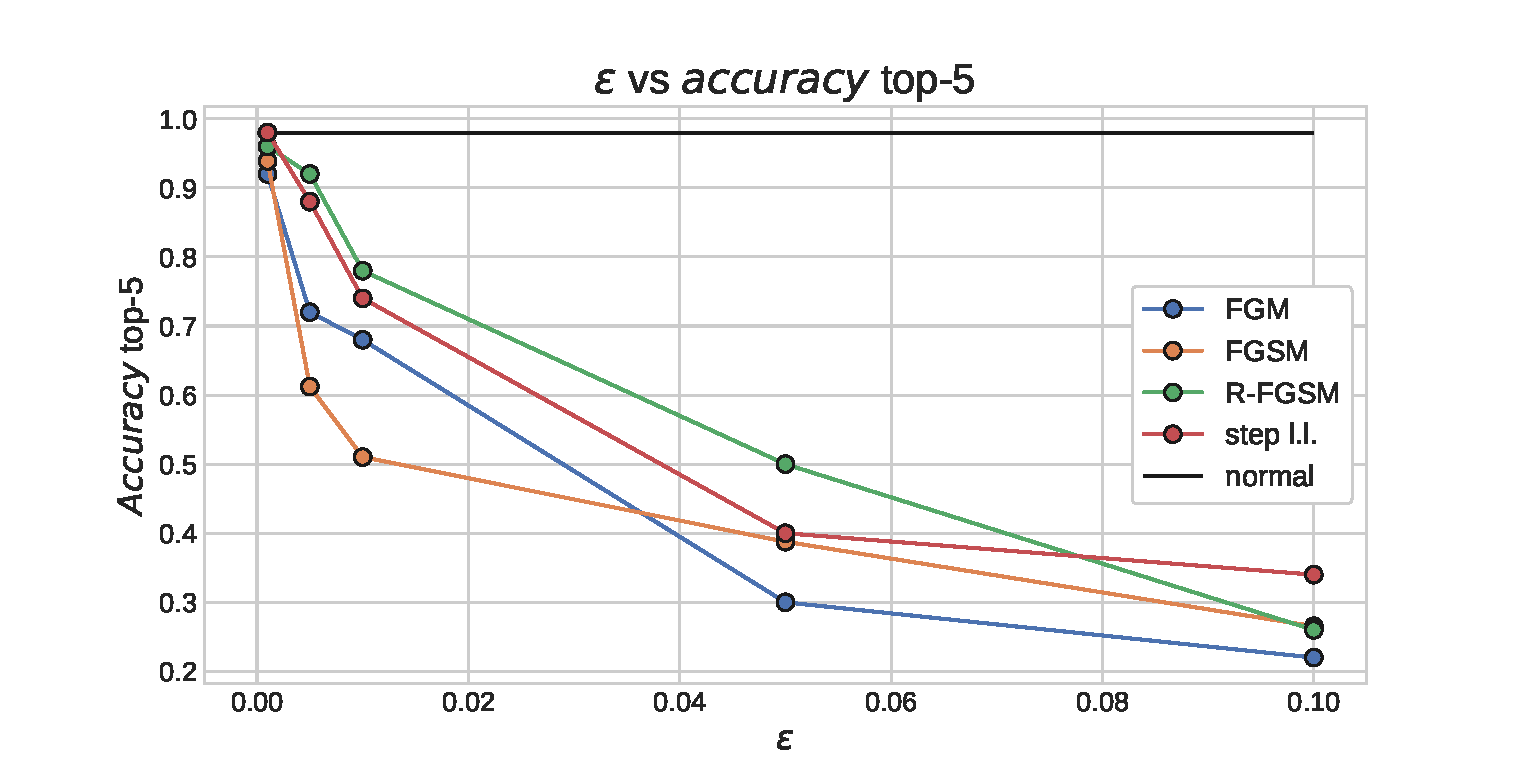
\includegraphics[width=\linewidth]{accuracy_top5.eps}
    \caption{\textit{Accuracy} top-5 contra $\epsilon$, para conjunto de 50 imágenes.}
    \label{fig:accuracytop5}
\end{figure}
En este experimento se considera el modelo \textit{ResNet50} pre-entrenado sobre \textit{ImageNet}. Luego, sobre él se ejecutarán ataques adversarios con un conjunto de imágenes, con el fin de observar como varía el \textit{accuracy} top-1 y \textit{accuracy} top-5 al pasar imágenes que han sido alteradas con el fin de engañar a la red. 

Los ataques considerados son los descritos en la sección de generación adversaria, luego, se observa que para todos los métodos a excepción de \textit{DeepFool}, se cuenta con un hiperparámetro $\epsilon$. Luego, se visualizará como cambia el \textit{accuracy} del modelo al variar este hiperparámetro. Se nota además que el método \textit{R-FGSM} requiere de otro hiperparámetro $\alpha$, el cual, para las experimentos de esta sección que lo requieran, será $\alpha = \frac{\epsilon}{2}$. Además, no se considera el método \textit{DeepFool} en este experimento dado que por definición este algoritmo itera hasta engañar al modelo, además de no contar con un hiperparámetro análogo a $\epsilon$ como los otros modelos.

En términos de especificaciones, se consideró el costo computacional que implica obtener ejemplos adversarios a partir de un modelo y un método, luego, para poder obtener resultados en un tiempo razonable y ajustándose a la disponibilidad de hardware, se decidió que las métricas de \textit{accuracy} serían computadas para un conjunto de 50 imágenes, las cuales son tomadas de 50 clases distintas. 

Teniendo lo anterior en consideración, se determinó de manera experimental el intervalo de variación de $\epsilon$ donde se observaban cambios relevantes, los valores a utilizar son:
\[
\epsilon \in \{0,001 ; 0,005 ; 0,01 ; 0,05 ; 0,1 \}
\]

Luego, para cada una de las 50 imágenes, se calcula su respectivo ejemplo adversario con los métodos descritos y se guarda la clase predicha, de esta manera, al realizar esto para todas las imágenes, para todos los valores de $\epsilon$ y para todos los ataques mencionados, se obtiene el cambio en el \textit{accuracy top-1} y \textit{accuracy top-5}.

\begin{table}[!t]
    \centering
    \caption{Accuracy Top-1 sobre conjunto de 50 imágenes al variar el hiperparámetro $\epsilon$ para distintos ataques.}
    \label{adv_top1_table}
    \begin{tabular}{cccccc} 
    \toprule 
     & \multicolumn{5}{c}{$\bm{\epsilon}$} \\ \cmidrule{2-6}
    \textbf{Ataque} & $0.001$ & $0.005$ & $0.01$ & $0.05$ & $0.1$ \\ \midrule
    FGSM & 0,65 & 0,26 & 0,18 & 0,14 & 0,04 \\ 
    FGM & 0,68 & 0,36 & 0,26 & 0,08 & 0,06 \\ 
    R-FGSM & 0,82 & 0,62 & 0,44 & 0,22 & 0,08 \\
    step l.l. & 0,82 & 0,54 & 0,46 & 0,24 & 0,20 \\ \bottomrule
    \end{tabular}
\end{table}

\begin{table}[!t]
    \centering
    \caption{Accuracy Top-5 sobre conjunto de 50 imágenes al variar el hiperparámetro $\epsilon$ para distintos ataques.}
    \label{adv_top5_table}
    \begin{tabular}{cccccc} 
    \toprule 
     & \multicolumn{5}{c}{$\bm{\epsilon}$} \\ \cmidrule{2-6}
    \textbf{Ataque} & $0.001$ & $0.005$ & $0.01$ & $0.05$ & $0.1$ \\ \midrule
    FGSM & 0,93 & 0,61 & 0,51 & 0,38 & 0,26 \\ 
    FGM & 0,92 & 0,72 & 0,68 & 0,30 & 0,22 \\ 
    R-FGSM & 0,96 & 0,92 & 0,78 & 0,50 & 0,26 \\
    step l.l. & 0,98 & 0,88 & 0,74 & 0,40 & 0,34 \\ \bottomrule
    \end{tabular}
\end{table}

\subsection{Análisis}

\begin{figure}[!tp]
    \centering
    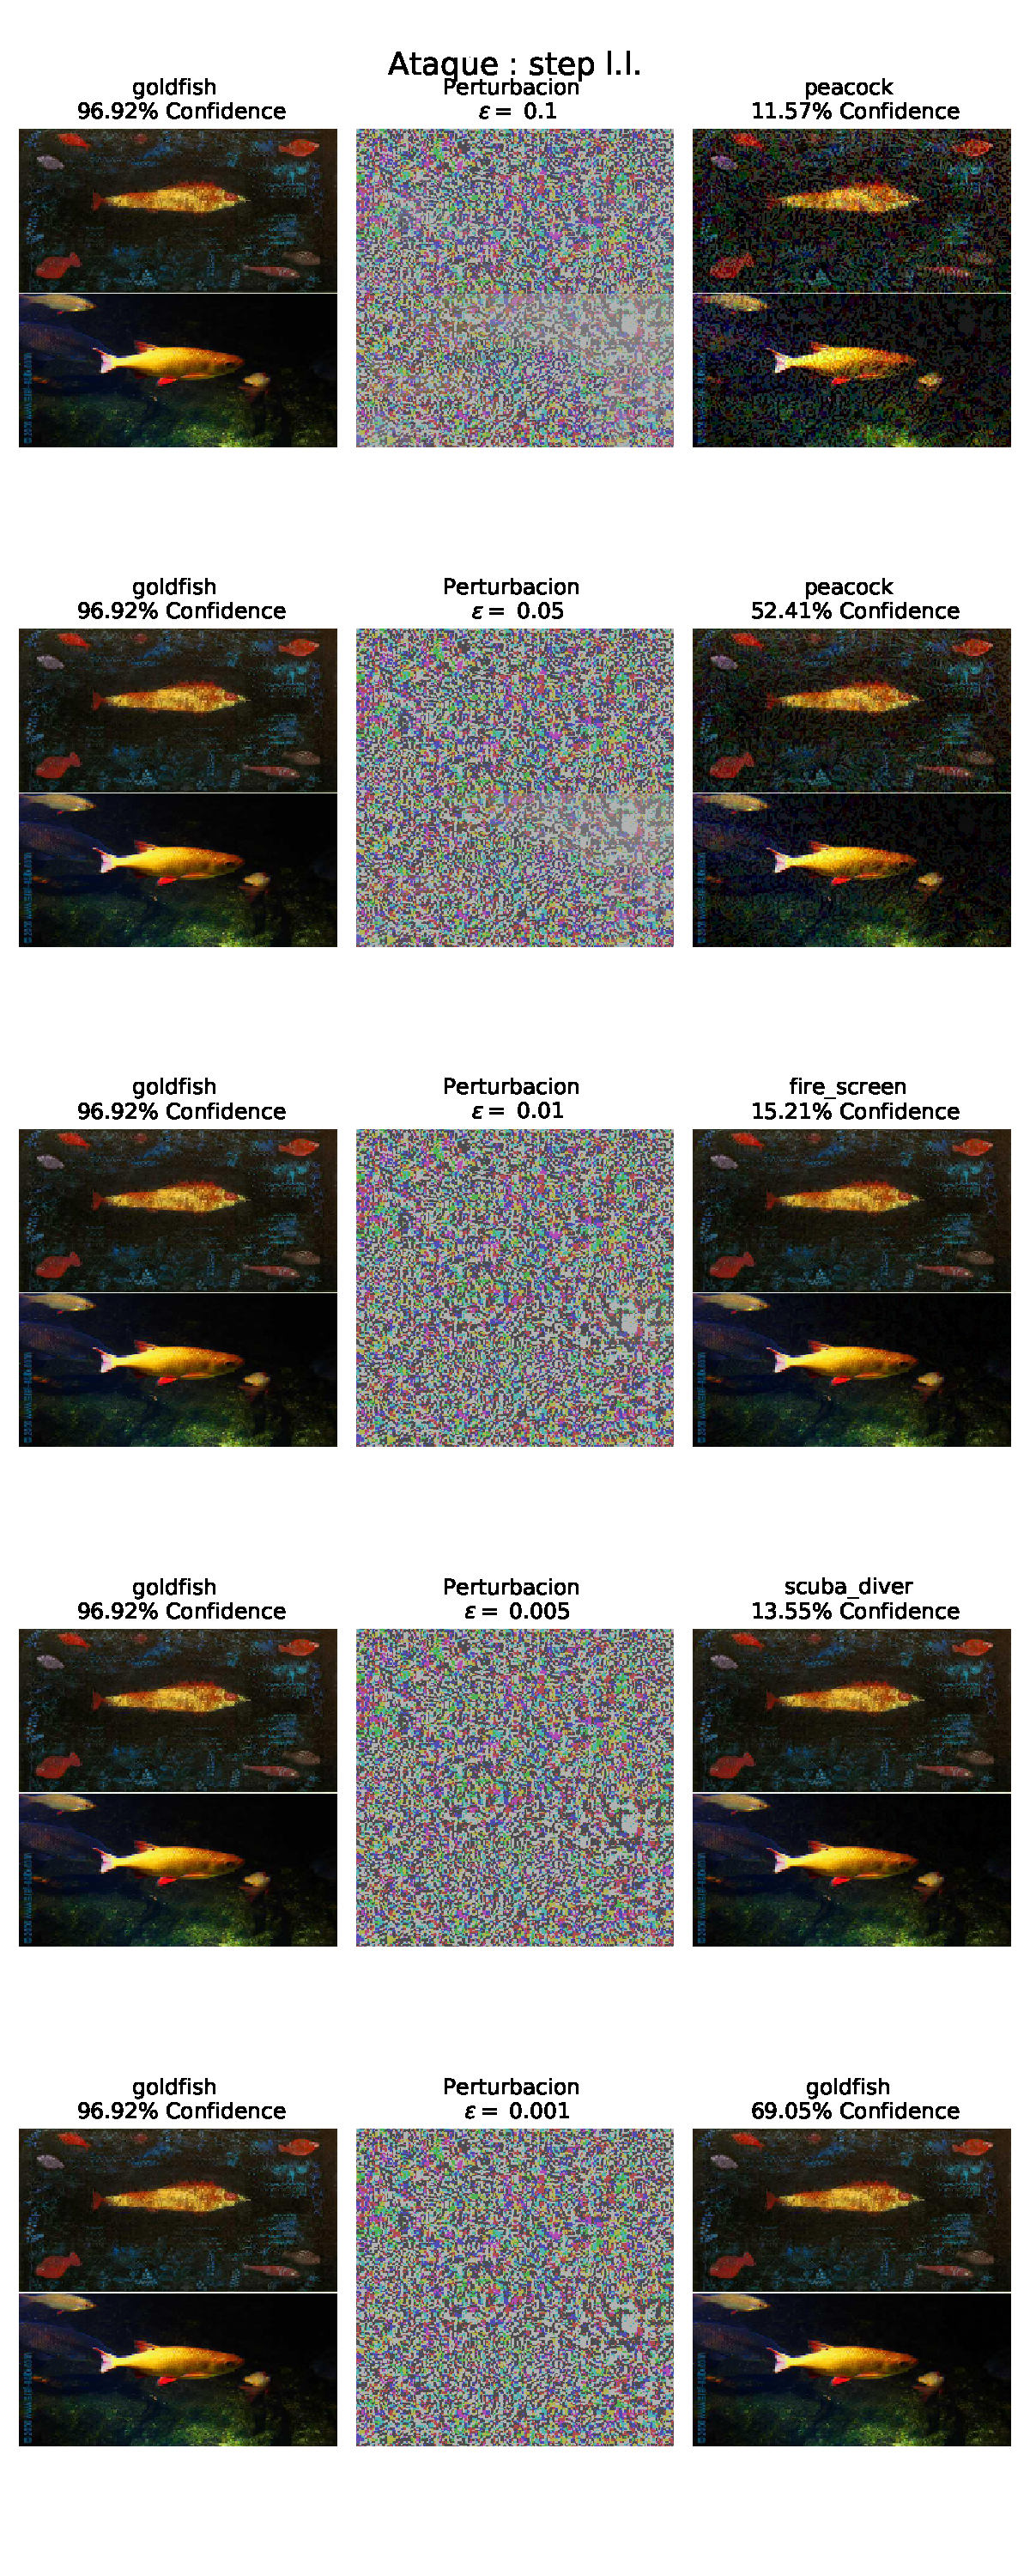
\includegraphics[width=\linewidth]{adv_2.pdf}
    \caption{Visualización de ataques adversarios utilizando el método \textit{step l.l.} con distinto factor de perturbación $\epsilon$ }
    \label{adv_comparison}
\end{figure}

De las Tablas \ref{adv_top1_table}, \ref{adv_top5_table} se observa en primer lugar que los ataques afectan más al \textit{accuracy} top-1, lo que es de esperarse dado que al utilizar ataques basados en gradiente se busca que el modelo prediga de manera incorrecta un ejemplo, lo que implica no ser la predicción con mayor confianza, pero nada asegura que un ejemplo pueda encontrarse dentro de los siguientes cuatro valores más probables. Por tanto, un primer resultado es que los métodos estudiados deben aplicar un perturbación mayor para lograr afectar métricas más generales como el \textit{accuracy} top-5.

Por otro lado, al analizar las Figuras \ref{fig:accuracytop1}, \ref{fig:accuracytop5}, se nota una segunda característica interesante de los ataques, cuyos efectos se ven reflejados en ambas métricas de \textit{accuracy}. Se observa que en valores de $\epsilon$ más pequeños, pequeñas variaciones de éste se ven reflejados en mayor medida en el \textit{accuracy}, en cambio a medida que aumenta $\epsilon$ las variaciones no muestran en mismo decaimiento, es decir, medida que aumenta $\epsilon$ el \textit{accuracy} estanca su descenso. Esto se tiene en primer lugar porque las predicciones se acercan a un \textit{accuracy} de cero. En segundo lugar, esto permite ver que el modelo es poco resistente a los ataques adversarios dado que para pequeños aumentos de $\epsilon$ el \textit{accuracy} decae rápidamente.

A modo de ejemplo se muestra en la Figura \ref{adv_comparison} los resultados de variar el $\epsilon$. En la columna izquierda, se tiene la imagen original, mostrando además la clase que el modelo predice y con cuanta confianza lo hace, luego, en la columna derecha se tiene el resultado de aplicar el método \textit{step l.l.} para crear el ejemplo adversario, observando además la clase predicha en este caso y su confianza asociada, por último, en la columna central se tiene la perturbación aplicada a la imagen original para obtener el ejemplo adversario.

En todos los casos se observa que el resultado de aplicar la generación adversaria es hasta cierto punto imperceptible e, incluso cuando se puede notar cierta distorsión en la imagen, la clase sigue siendo clara. Pero para el modelo de clasificación esto no es así, dado que se observa que a excepción del caso con $\epsilon=0.001$ todos los otros fueron mal clasificados.

\bibliographystyle{./bibliography/IEEEtran}

\begin{thebibliography}{1}
\bibitem{deepdefense}
Z. Yan, Y. Guo y C. Zhang, “Deep Defense: Training DNNs with Improved Adversarial Robustness”, en  \textit{arXiv e-prints, arXiv:1803.00404}, febrero 2018.
\bibitem{goodfellow2013}
C. Szegedy, W. Zaremba, I. Sutskever, J. Bruna, D. Erhan, Dumitru, I. Goodfellow y R. Fergus, “Intriguing properties of neural networks” en \textit{arXiv e-prints, arXiv:1312.6199}, diciembre 2013.
\bibitem{evtimov2017}
I. Evtimov, K. Eykholt, E. Fernandes, T. Kohno, B. Li, A. Prakash, A. Rahmati y D. Song, “Robust physical-world attacks on deep learning models”, \textit{arXiv e-print, arXiv:1707.08945}, julio 2017.
\bibitem{kurakin2016physical}
A. Kurakin, I. Goodfellow y S. Bengio, “Adversarial examples in the physical world”, \textit{arXiv e-prints, arXiv:1607.02533}, julio 2016.

\bibitem{xie2017}
C. Xie, J. Wang, Z. Zhang, Y. Zhou, L. Xie y A. Yuille, “Adversarial examples for semantic segmentation and object detection”, en \textit{IEEE International Conference on Computer Vision (ICCV)}, 2017, pp. 1378-1387.

\bibitem{imagenet}
O. Russakovsky et al., ``ImageNet Large Scale Visual Recognition Challenge'', en \textit{arXiv e-prints, arXiv:1409.0575}, septiembre 2014.
\bibitem{goodfellow2014}
I. Goodfellow, J. Shlens y C. Szegedy, “Explaining and Harnessing Adversarial Examples” en \textit{arXiv e-prints, arXiv:1412.6572}, diciembre 2014.
\bibitem{kurakin2016}
A. Kurakin, I. Goodfellow y S. Bengio, ``Adversarial Machine Learning at Scale'', en \textit{arVix e-prints, arXiv:1611.01236}, noviembre 2016.
\bibitem{tramer2017}
F. Tramèr, A. Kurakin, N. Papernot, I. Goodfellow, D. Boneh y P. McDaniel, ``Ensemble Adversarial Training: Attacks and Defenses'', en \textit{arXiv e-prints, arXiv:1705.07204}, mayo 2017.
\bibitem{deepfool}
S.-M. Moosavi-Dezfooli, A. Fawzi y P. Frossard, “DeepFool: a simple and accurate method to fool deep neural networks”, en  \textit{arXiv e-prints, arXiv:1511.04599}, noviembre 2015.
\bibitem{yuan2017}
X. Yuan, P. He, Q. Zhu y X. Li, “Adversarial Examples: Attacks and Defenses for Deep Learning”, en \textit{arXiv e-prints, arXiv:1712.07107}, diciembre 2017.
\bibitem{foolbox}
J. Rauber, W. Brendel y M. Bethge, “Foolbox: A Python toolbox to benchmark the robustness of machine learning models”, en \textit{arXiv e-prints, arXiv:1707.04131}, julio 2017.
\bibitem{resnet}
K. He, X. Zhang, S. Ren y J. Sun, ``Deep Residual Learning for Image Recognition'' en \textit{arXiv e-prints, arXiv:1512.03385}, diciembre 2015.
\bibitem{vgg16}
K. Simonyan,  A. Zisserman, ``Very Deep Convolutional
Networks For Large-Scale Image Regcognition'', en \textit{arXiv e-print, arXiv:1409.1556}, abril 2015.
\end{thebibliography}

\end{document}
